\section{РЕЗУЛЬТАТЫ ЖАНРОВОЙ КЛАССИФИКАЦИИ}
\label{sec:genre_classification}


Для проверки значимости выделенных образов было принято решения проверить их на задаче жанровой классификации. 

В качестве исходной выборки был использован репозиторий GZTAG. Набор данных состоит из 1000 звуковых дорожек каждые по 30 секунд. Он содержит 10 жанров, каждый из которых представлен 100 треками. Все треки - это все 220-мегагерцовые Mono 16-битные аудиофайлы в формате .wav.


Для решения задачи классификации была использована библиотека scikit-learn -- бесплатная библиотека для машинного обучения с открытым исходным кодом для языка программирования Python. Все методы классификации использованы с параметрами по умолчанию. 

\subsection{AdaBoost с деревьями принятия решений}

AdaBoost zвляется мета-алгоритмом, в процессе обучения строит композицию из базовых алгоритмов обучения для улучшения их эффективности. AdaBoost является алгоритмом адаптивного бустинга в том смысле, что каждый следующий классификатор строится по объектам, которые плохо классифицируются предыдущими классификаторами.

AdaBoost вызывает слабый классификатор в цикле. После каждого вызова обновляется распределение весов, которые отвечают важности каждого из объектов обучающего множества для классификации. На каждой итерации веса каждого неверно классифицированного объекта возрастают, таким образом новый классификатор <<фокусирует своё внимание>> на этих объектах.

В качестве слабого классификаторы было использованно дерево принятие решений. Максимальное количество слабых классификаторов установлено в количестве 50. В качестве алгоритма обучения использовался алгоритм SAMME.


Как показывает рисунок \ref{fig:results:adaboost} данный классификатор плохо справляется с задачей классификации. Классифицировались фрагменты по 5 секунд с перекрытием в 0,5 секунд. Из жанров лучше всего классифицировались классическая музыка -- 70 \%, металл -- 47 \% и хипхоп -- 49 \%. 

Оценка перекрёстной проверки с десятью разбиениями -- 28 \% cо средней квадратичным отклонением 3,8 \%.  

Для задачи жанровой классификации данный метод с текущими параметрами и с теми выделенными образами для решения задачи жанровой классификации не подходит. 

\begin{figure}[h]
\centering
  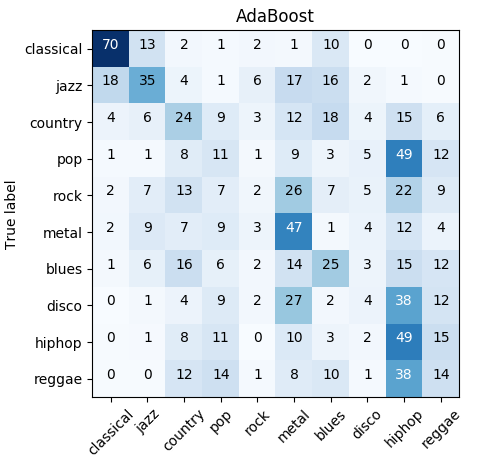
\includegraphics{AdaBoost.png}
  \caption{Матрица ошибок для фрагмента трека  полученная с помощь метода классификации AdaBoost SAMME, где используется <<комитет>>  деревьев принятия решений.}
  \label{fig:results:adaboost}
\end{figure}

\subsection{Дерево принятия решений}

Деревья принятия решений - это непараметрический контролируемый метод обучения, используемый для классификации и регрессии. Цель состоит в том, чтобы создать модель, которая предсказывает значение целевой переменной путем изучения простых правил принятия решений, выведенных из данных.

В качестве алгоритма обучения используется оптимизированная версия CART. В качестве индекса неоднородности используется индекс Джини. Максимальная глубина дерева ограничена до 5 уровней.

Как показывает рисунок \ref{fig:results:DecisionTree} дерево принятия решений смогло выделить все классы, что видно по главной диагонали матрицы ошибок. Лучше всего распознались следующие жанры: классическая музыка -- 61 \%, джаз -- 56 \%, поп -- 50 \% и метал -- 58 \%. Хуже всего: диско -- 29 \%, рок -- 25 \%. 


Оценка перекрёстной проверки с десятью разбиениями -- 42 \% cо средней квадратичным отклонением 4 \%.  

\begin{figure}[h]
\centering
  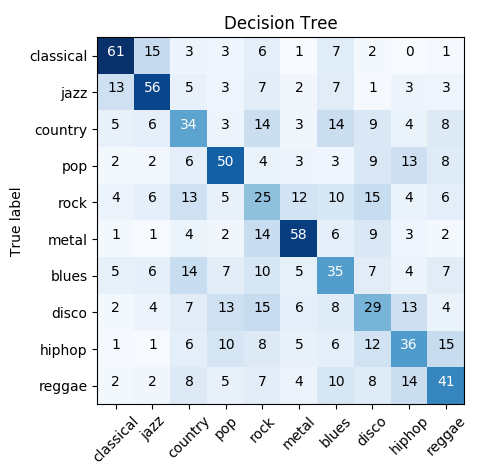
\includegraphics{DecisionTree.png}
  \caption{Матрица ошибок для фрагмента трека полученная с помощь дерева принятия решения}
  \label{fig:results:DecisionTree}
\end{figure}

При классификации всего трека использовалась интегрированная оценка по всем фрагментам. Класс трека определялся наиболее часто встречаемым предсказанным классом его фрагментов. Это улучшило результаты классификации, как можно видеть на рисунке \ref{fig:results:DecisionTree1}. 

\begin{figure}[h]
\centering
  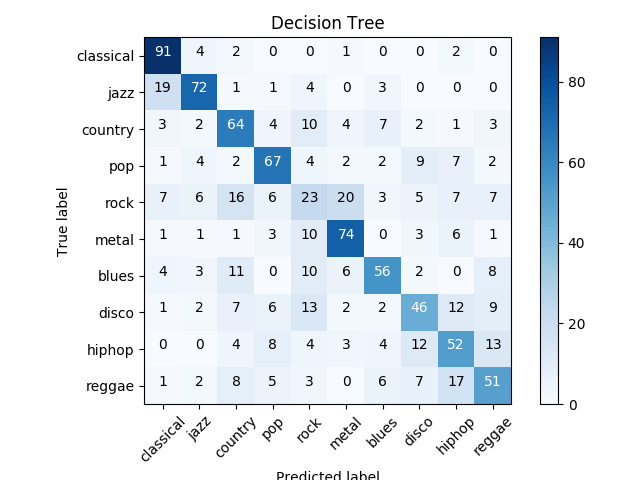
\includegraphics{DecisionTree_new1.png}
  \caption{Матрица ошибок для всего трека  полученная с помощь дерева принятия решения}
  \label{fig:results:DecisionTree1}
\end{figure}


\subsection{Метод опорных векторов}

Метод опорных векторов --  набор схожих алгоритмов обучения с учителем, использующихся для задач классификации и регрессионного анализа. Принадлежит семейству линейных классификаторов и может также рассматриваться как специальный случай регуляризации по Тихонову. Особым свойством метода опорных векторов является непрерывное уменьшение эмпирической ошибки классификации и увеличение зазора, поэтому метод также известен как метод классификатора с максимальным зазором.

Основная идея метода -- перевод исходных векторов в пространство более высокой размерности и поиск разделяющей гиперплоскости с максимальным зазором в этом пространстве. Две параллельных гиперплоскости строятся по обеим сторонам гиперплоскости, разделяющей классы. Разделяющей гиперплоскостью будет гиперплоскость, максимизирующая расстояние до двух параллельных гиперплоскостей. Алгоритм работает в предположении, что чем больше разница или расстояние между этими параллельными гиперплоскостями, тем меньше будет средняя ошибка классификатора.

\begin{figure}[h]
\centering
  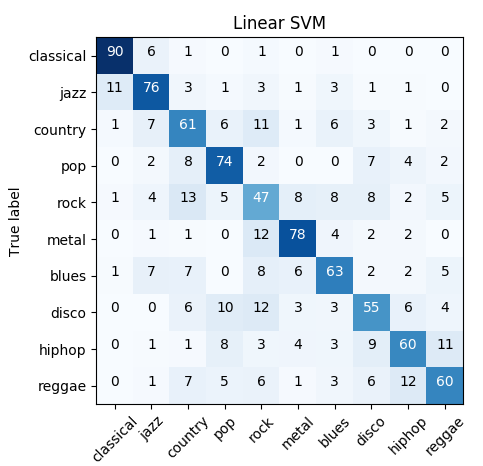
\includegraphics{LinearSVM.png}
  \caption{Матрица ошибок для фрагмента трека   полученная с помощь метода опорных векторов}
  \label{fig:results:LinearSVM}
\end{figure}

Как показывает рисунок \ref{fig:results:LinearSVM} метод опорных векторов отлично справляется с задачи жанровой классификации. 


Оценка перекрёстной проверки с десятью разбиениями -- 66,3 \% cо средне квадратичным отклонением 0,23 \%.  

При классификации всего трека (см рисунок \ref{fig:results:LinearSVM_new}) обобщающая способность метода составила 76 \%. 

\begin{figure}[h]
\centering
  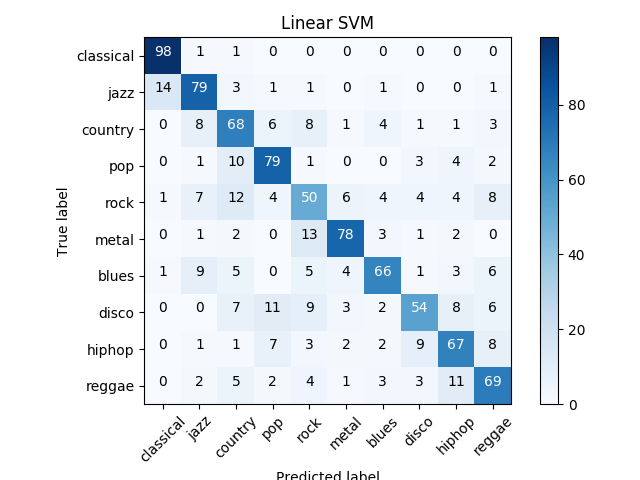
\includegraphics{LinearSVM_new.png}
  \caption{Матрица ошибок  для всего трека полученная с помощь метода опорных векторов}
  \label{fig:results:LinearSVM_new}
\end{figure}


\subsection{Наивный баесовский классификатор}

Наивный байесовский классификатор -- простой вероятностный классификатор, основанный на применении Теоремы Байеса со строгими (наивными) предположениями о независимости.

В зависимости от точной природы вероятностной модели, наивные байесовские классификаторы могут обучаться очень эффективно. Во многих практических приложениях для оценки параметров для наивных байесовых моделей используют метод максимального правдоподобия; другими словами, можно работать с наивной байесовской моделью, не веря в байесовскую вероятность и не используя байесовские методы.

Несмотря на наивный вид и, несомненно, очень упрощенные условия, наивные байесовские классификаторы часто работают намного лучше во многих сложных жизненных ситуациях.

Достоинством наивного байесовского классификатора является малое количество данных для обучения, необходимых для оценки параметров, требуемых для классификации.

Как показывает рисунок \ref{fig:results:NaiveBayes} наивный баесовский классификатор смог выделить все классы, что видно по главной диагонали матрицы ошибок. Лучше всего распознались следующие жанры: классическая музыка -- 81 \%, металл -- 77 \%, диско -- 59 \% . Хуже всего: хипхоп -- 10 \% и рок -- 11 \%.  Рок чаще всего идентифицируется как кантри, металл или диско.

Оценка перекрёстной проверки с десятью разбиениями -- 47,8 \% cо средне квадратичным отклонением 3 \%.  

\begin{figure}[h]
\centering
  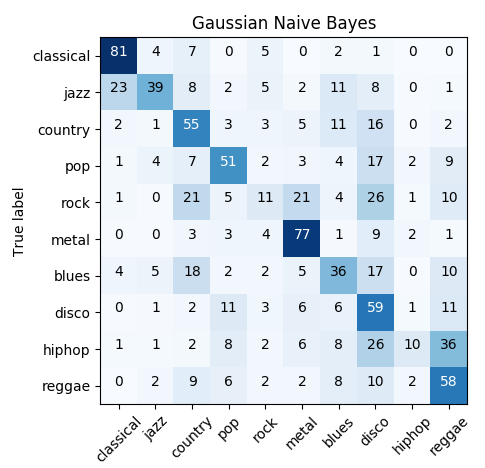
\includegraphics{NaiveBayes.png}
  \caption{Матрица ошибок  для фрагмента трека полученная с помощь наивного баесовского классификатора}
  \label{fig:results:NaiveBayes}
\end{figure}

При классификации всего трека (см рисунок \ref{fig:results:NaiveBayes_new}) обобщающая способность метода составила 52 \%. 

\begin{figure}[h]
\centering
  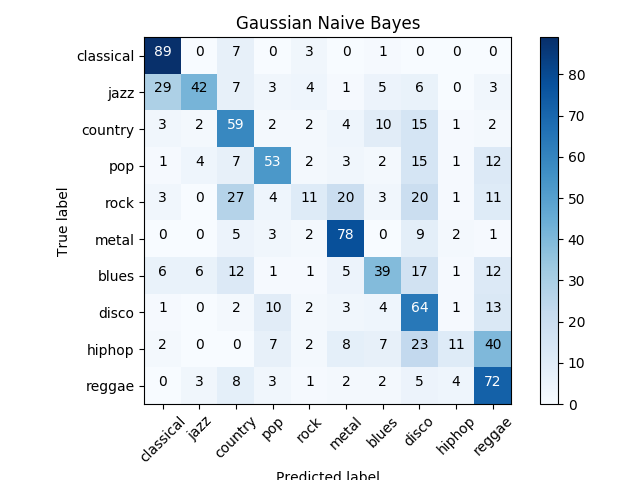
\includegraphics{NaiveBayes_new.png}
  \caption{Матрица ошибок  для всего трека полученная с помощь наивного баесовского классификатора}
  \label{fig:results:NaiveBayes_new}
\end{figure}

\subsection{Метод ближайших соседей}

Метод k ближайших соседей -- метрический алгоритм для автоматической классификации объектов. Основным принципом метода ближайших соседей является то, что объект присваивается тому классу, который является наиболее распространённым среди соседей данного элемента.

Соседи берутся исходя из множества объектов, классы которых уже известны, и, исходя из ключевого для данного метода значения k высчитывается, какой класс наиболее многочислен среди них. Каждый объект имеет конечное количество атрибутов (размерностей).

Предполагается, что существует определенный набор объектов с уже имеющейся классификацией.

Как показывает рисунок \ref{fig:results:NearestNeighbors} метод ближайших соседей смог выделить все классы, что видно по главной диагонали матрицы ошибок. Лучше всего распознались следующие жанры: классическая музыка -- 86 \%, металл -- 74 \%, поп -- 64 \% . Хуже всего: блюз -- 38 \% и хипхоп -- 28 \%. Также заметна сильная погрешность при классификации  джаза -- 32 \% фрагментов этого жанра было отнесено к классической музыке. Изменение числа соседей приводило к лучшей классификации металла, классической и поп музыки. 

Оценка перекрёстной проверки с десятью разбиениями -- 50,6 \% cо средне квадратичным отклонением 2,5 \%.  

\begin{figure}[h]
\centering
  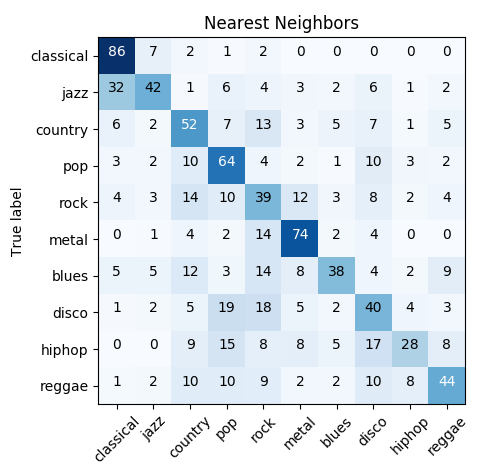
\includegraphics{NearestNeighbors.png}
  \caption{Матрица ошибок для фрагмента трека полученная с помощь метода k ближайших соседей}
  \label{fig:results:NearestNeighbors}
\end{figure}

При классификации всего трека (см рисунок \ref{fig:results:NearestNeighbors_new}) обобщающая способность метода составила 69 \%. 

\begin{figure}[h]
\centering
  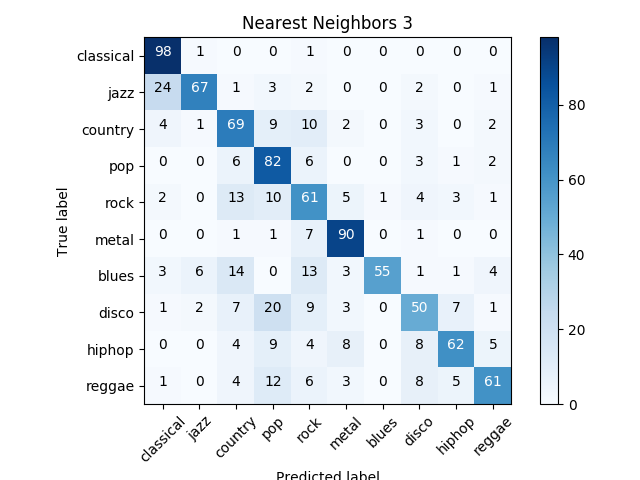
\includegraphics{NearestNeighbors_new1.png}
  \caption{Матрица ошибок  для всего трека  полученная с помощь метода k ближайших соседей}
  \label{fig:results:NearestNeighbors_new}
\end{figure}



\subsection{Многослойный персептрон}


Многослойными персептронами называют нейронные сети прямого распространения. Входной сигнал в таких сетях распространяется в прямом направлении, от слоя к слою. Многослойный персептрон в общем представлении состоит из следующих элементов:
\begin{itemize}
\item    множества входных узлов, которые образуют входной слой;
\item    одного или нескольких скрытых слоев вычислительных нейронов;
\item    одного выходного слоя нейронов.
\end{itemize}
Многослойный персептрон представляет собой обобщение однослойного персептрона Розенблатта.

В данной задачи использовался один скрытый слой с 1000 нейронами. В качестве функции активации использовалась положительно полулинейная функция.

\begin{figure}[h]
\centering
  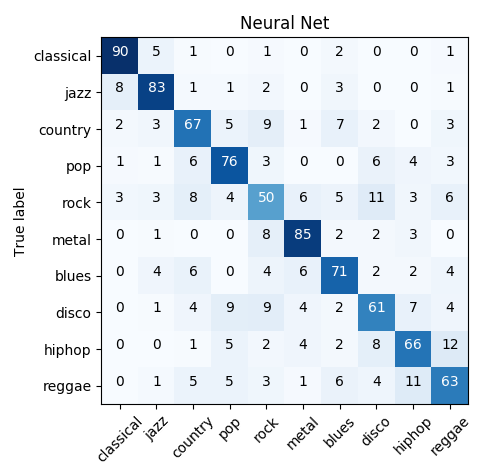
\includegraphics{NeuralNet.png}
  \caption{Матрица ошибок для фрагмента трека полученная с помощь многослойного перцептрона}
  \label{fig:results:NeuralNet}
\end{figure}

Как показывает рисунок \ref{fig:results:NeuralNet} многослойный перцептрон смог выделить все классы, что видно по главной диагонали матрицы ошибок. Данный метод классификации показал наилучшие результаты. Качество распознования по всем классам не ниже 50 процентов.

Оценка перекрёстной проверки с десятью разбиениями -- 71 \% cо средне квадратичным отклонением 2,5 \%

При классификации всего трека (см рисунок \ref{fig:results:NeuralNet_new}) обобщающая способность метода составила 81 \%. Качество распознования увеличилось по всем классам, кроме рока. 

\begin{figure}[h]
\centering
  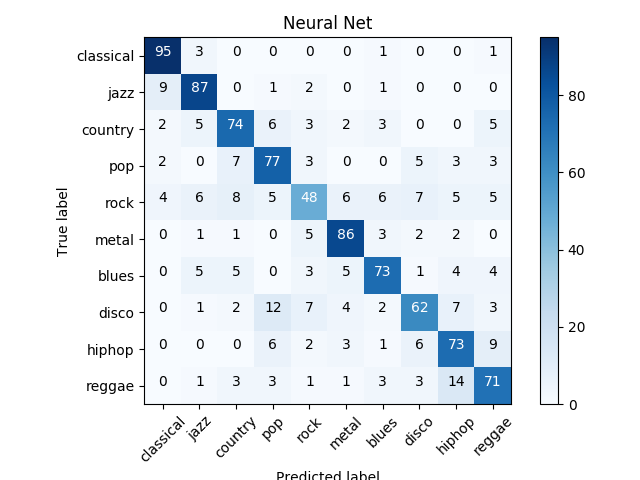
\includegraphics{NeuralNet_new.png}
  \caption{Матрица ошибок  для всего трека  полученная с помощь многослойного перцептрона}
  \label{fig:results:NeuralNet_new}
\end{figure}



\subsection{Квадратичный дискриминант}


Квадратичный дискриминант - это вариант Байесовского классификатора, который основывается на двух дополнительных допущениях, касающихся вероятностных свойств выборки, а именно - независимость выборки и ее нормальность. Нормальное (гауссово) распределение широко используется по причине вычислительного удобства и адекватности во многих случаях. 

\begin{figure}[h]
\centering
  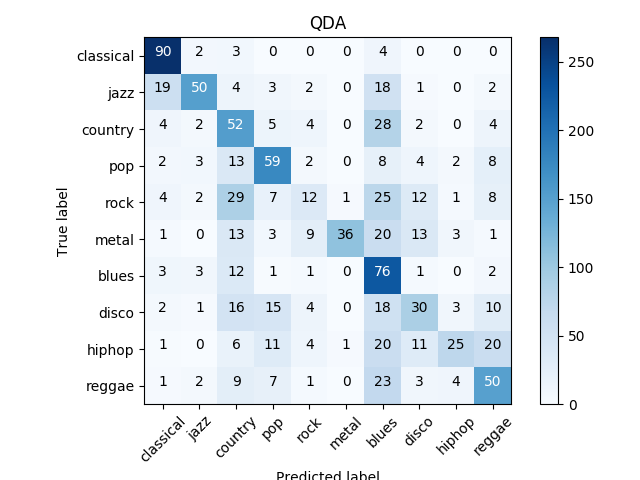
\includegraphics{QDA.png}
  \caption{Матрица ошибок для фрагмента трека полученная с помощь QDA}
  \label{fig:results:QDA}
\end{figure}

Как показывает рисунок \ref{fig:results:QDA} при достаточно хорошей оценки перекрёстной проверки видно, что сам метод классификации не подходит, так как 20 \% ошибок на других жанрах он классифицирует как блюз. 

При классификации всего трека (см рисунок \ref{fig:results:QDA_new}) обобщающая способность метода составила 51 \%. 
\begin{figure}[h]
\centering
  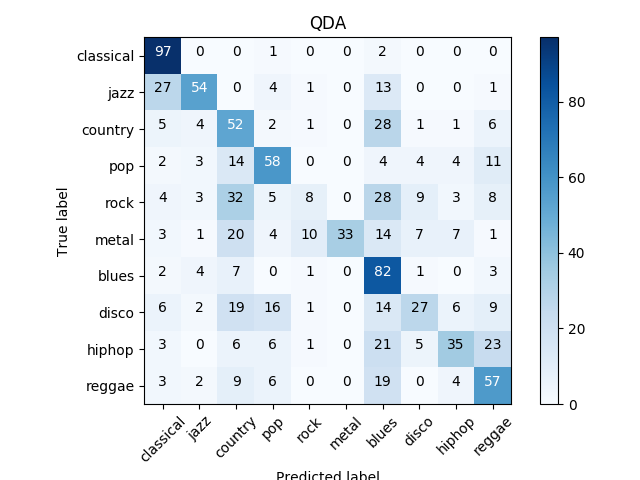
\includegraphics{QDA_new.png}
  \caption{Матрица ошибок для всего трека полученная с помощь QDA}
  \label{fig:results:QDA_new}
\end{figure}


\subsection{Случайный лес}

Случайный лес -- алгоритм машинного обучения, предложенный, заключающийся в использовании комитета (ансамбля) решающих деревьев. Классификация объектов проводится путём голосования: каждое дерево комитета относит классифицируемый объект к одному из классов, и побеждает класс, за который проголосовало наибольшее число деревьев.

Оптимальное число деревьев подбирается таким образом, чтобы минимизировать ошибку классификатора на тестовой выборке. В случае её отсутствия, минимизируется оценка ошибки out-of-bag: доля примеров обучающей выборки, неправильно классифицируемых комитетом, если не учитывать голоса деревьев на примерах, входящих в их собственную обучающую подвыборку.

\begin{figure}[h]
\centering
  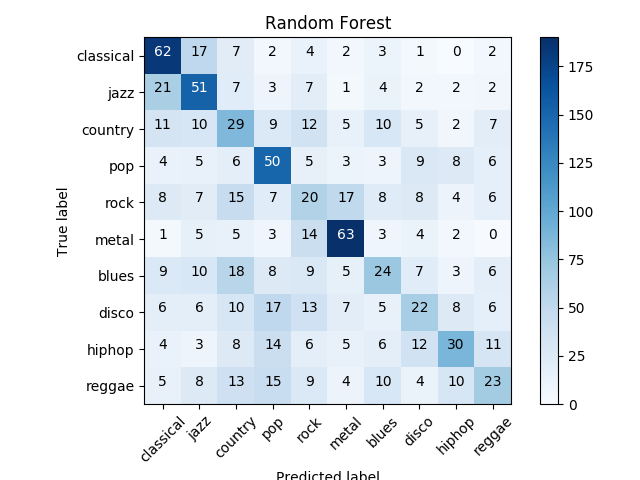
\includegraphics{RandomForest.png}
  \caption{Матрица ошибок для фрагмента полученная с случайного леса}
  \label{fig:results:RandomForest}
\end{figure}

Оценка перекрёстной проверки с десятью разбиениями -- 39 \% cо средне квадратичным отклонением 3 \%

При классификации всего трека (см рисунок \ref{fig:results:QDA_new}) обобщающая способность метода составила 54 \%. 
\begin{figure}[h]
\centering
  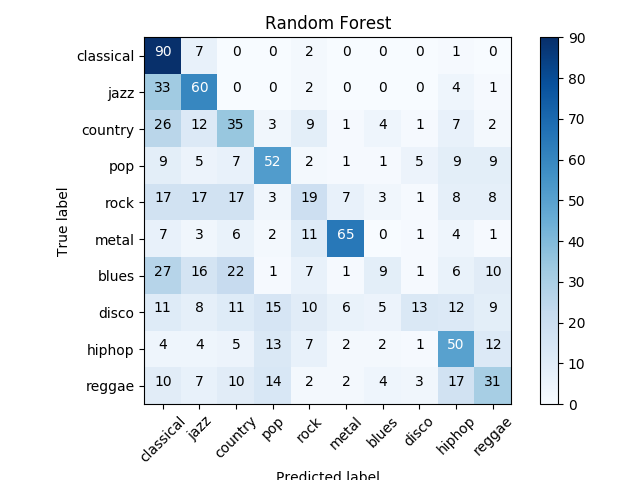
\includegraphics{RandomForest_new.png}
  \caption{Матрица ошибок  для всего трека полученная с помощь QDA}
  \label{fig:results:RandomForest_new}
\end{figure}


В результате даже самые элементарные алгоритмы классификации показали свою эффективность, что показывает, что выделенные информационные образы значимы и могут быть использованны в системах рекомендации музыки. Лучше всего распозналась музыка в жанре поп, металл и классическая музыка. Хуже всего рок.  Все результаты сведены в таблицу
\ref{table:result:result}.



\begin{table}[h]
\caption{Таблица результатов классификации}
\label{table:result:result}
  \centering
  \begin{tabular}{| >{\raggedright}m{0.35\textwidth}
                  | >{\centering}m{0.25\textwidth}
                  | >{\centering\arraybackslash}m{0.25\textwidth}|}
    \hline
    {\begin{center}
    Методы классификации
    \end{center} } &  фрагмент 5 сек. перекрытие 0.1 \% &  Трек, на основе фрагмента 5 сек. перекрытие 0.5 \%  \\
    
    \hline
    
    AdaBoost с деревьями принятия решений & \num{28,2} & \num{44}  \\
    
    \hline

    Дерево принятия решений & \num{42,4} & \num{59}  \\

    \hline

    Метод опорных векторов & \num{66,3} & \num{76}   \\

    \hline

    Наивный баесовский классификатор & \num{47,8} & \num{52} \\

    \hline

    Метод ближайших соседей & \num{50,6} & \num{69} \\

    \hline

    Нейронная сеть прямого распространения & \num{71,0} & \num{81} \\

    \hline
    
    Квадратичный дискриминант & \num{47,9} & \num{51} \\

    \hline

    Случайный лес & \num{39,0} & \num{52}  \\

    \hline

  \end{tabular}
\end{table}





